% !TEX root = ../../semexp-thesis.tex

\section{Prototyping User Interfaces with Semantic Suggestions and Completions}
\label{sec:application/suggestions}

In this case study, we describe how a programmer builds a prototype for a simple counter application in the Morphic framework of Squeak with the help of semantic suggestions and completions.

To start the exploration, the programmer opens a workspace, types in a simple do-it for creating and showing a simple morph (i.e., a graphical object), and executes it:

\begin{center}
	\begin{tblr}{
		colspec={X[2.5,m] X[1,m]},
		colsep=0.5em,
		rowsep=0pt,
		column{1}={leftsep=0pt},
		column{2}={rightsep=0pt},
	}
		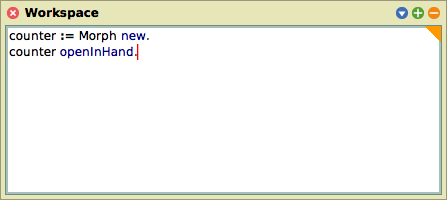
\includegraphics[width=\linewidth]{01_suggestions/workspace_start.png} & % TODO screenshot: [COULD] improve resolution, maybe scale down workspace
		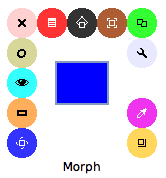
\includegraphics[width=\linewidth]{01_suggestions/app_start.png} % TODO screenshot: [COULD] improve resolution
	\end{tblr}
	\captionof{figure}{Bootstrapping the prototyping of a Morphic UI application in a workspace.}
\end{center}

As the programmer is viewing the plain default morph and the workspace is ready for further experiments, the programmer wonders about the different possibilities for visual customization that th morph offers.
Traditionally, answering this question would require them to browse the available protocols of the morph, check out the documentation of the class, or research different samples of similar existing Morphic applications.

However, once the programmer has entered the do-it, the \emph{suggestion space} has already conducted plenty of such research in the background and now displays a summary of information about the morph's interface:
in a list, the programmer can view different common selectors for modifying the appearance, layout, or composition of the morph.
For each selector, the suggestion space displays the parameter signature of the message, any available documentation from the \code{Morph} class, and a short list of example usage snippets from other packages in the system:

\noindent
\begin{minipage}{\textwidth}
	\centering
	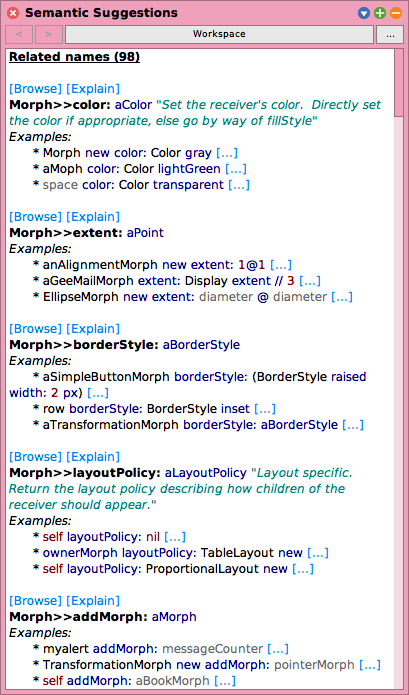
\includegraphics[height=28\baselineskip]{01_suggestions/suggestion_space.png} % TODO screenshot: [COULD] improve resolution
	\captionof{figure}[Using the suggestion space to browse relevant protocols of the class \code{Morph} for prototyping a user interface.]{
		Using the suggestion space to browse relevant protocols of the class \code{Morph} for prototyping a user interface.
	}
\end{minipage}

Within this list, the programmer discovers the \code{\#color:} selector and decides to adjust the color of their counter morph.
To achieve that, they simply reuse one of the included usage examples and apply it in the workspace (\code{counter color: Color gray}).
Analogously, they change the size of the morph by adding an \code{\#extent:} message send.
Thus, the programmer was able to answer their question about relevant protocols of the morph without searching the interfaces of the \code{Morph} class manually, seek inspiration from automatically collected examples, and understand how to use these protocols through the context of the provided documentation and usage snippets.

Next, the programmer wishes to add a border to the morph.
From the examples in the suggestion space, they understand that borders can be configured through the \code{\#borderStyle:} selector, but they do not yet comprehend all the different options that are available through the argument of this selector.
Nevertheless, they begin by already typing an incomplete message send with that selector into their workspace.
Traditionally, they now would be required to browse further examples or documentation related to this selector to learn more about possible arguments that can be passed.

However, the \emph{semantic autocompletion} has detected the intent of the programmer through their typed prefix and automatically suggests different possible border styles in the completion menu of the text interface.
Each border style is given through a different argument expression, exhibits different visual features such as width, dashes, and skeuomorphisms, and is displayed with a graphical preview of applying this style to the counter morph:

\begin{center}
	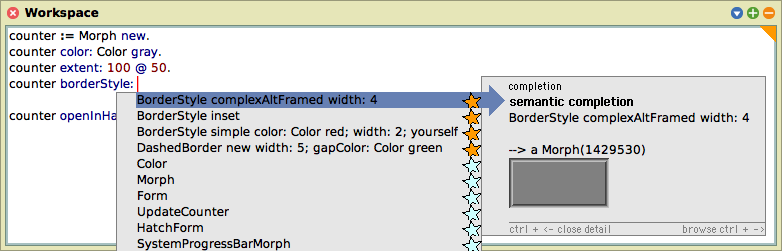
\includegraphics[width=\linewidth]{01_suggestions/semantic_autocompletion.png} % TODO screenshot: [COULD] improve resolution
	\captionof{figure}[Using the semantic autocompletion to explore different customization possibilities for borders of our Morphic UI prototype.]{
		Using the semantic autocompletion to explore different customization possibilities for borders of our Morphic UI prototype.
	}
\end{center}

The programmer can browse these completion suggestions to inspect the generated code, related documentation from the used classes and messages, and their effect, and accept any completion to insert it into the workspace.
Thus, the programmer could explore and compare different possible designs based on the available interfaces while avoiding to manually browse existing usage samples, combine them, or transfer them to the context of their own script.

In a similar manner, the programmer can also proceed to add a label and a button to the counter morph.
As the general overview in the suggestion space currently does not show any suggestions to these specific widgets, they start by explicating their intent through a comment in the workspace (\code{\textquotedbl add label and button\textquotedbl}).
In response, the suggestion space and the semantic autocompletion provide them with suggestions for different types and layouts of labels and buttons for the counter morph.

After the programmer has chosen and applied any of these suggestions, the final step is to make their prototype functional by adding behavior to the button.
To this end, they start by defining a new counter variable.
Automatically, the semantic autocompletion scans the available protocols of the used widgets and suggests different code snippets that will trigger an increment of the counter variable and an update in the label for every click on the button.
Again, the programmer compares the different implementations, chooses their prefered option, and executes it in the workspace to complete their first prototype of the counter application:

\begin{center}
	\begin{tblr}{
		colspec={X[2.5,m] X[1,m]},
		colsep=0.5em,
		rowsep=0pt,
		column{1}={leftsep=0pt},
		column{2}={rightsep=0pt},
	}
		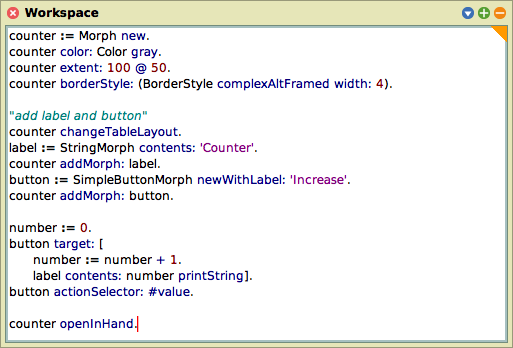
\includegraphics[width=\linewidth,valign=c]{01_suggestions/workspace_final.png} & % TODO screenshot: [COUD] improve resolution, slightly shrink workspace horizontally?
		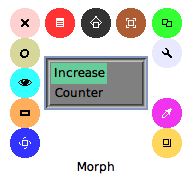
\includegraphics[width=\linewidth,valign=c]{01_suggestions/app_final.png} % TODO screenshot: [COULD] improve resolution
	\end{tblr}
	\captionof{figure}{The complete prototype of our Morphic counter application in Squeak.}
\end{center}

In summary, the programmer could build a UI prototype in a more fluent process, spend less time, and achieve a better-grounded result by using semantic suggestions and semantic completions.
They could remain in their flow of conceptualizing a UI design without being disrupted by having to manually research extensive interfaces and documentation or read and comprehend many incoherent and redundant examples.
They could improve the quality of their prototype by considering suggestions based on a larger number of sources and comparing multiple distilled, distinct options with regard to their inner (code) quality and their visible effect.
